\chapter{生物分子：氨基酸、糖、脂质与核苷酸}\label{ch:b2:biomolecules}

一种常见甜味剂，甜度远高于蔗糖，由两个氨基酸经单个酰胺键连接而成，其中
一个为甲酯：即天冬氨酸与苯丙氨酸，两者均具有活细胞所用的构型。
生命分子由几类小单元构成：氨基酸、糖、
脂肪酸和核苷酸，经由前几章的反应连接在一起：酰胺、缩醛、酯。本章
以有机化学家的视角审视它们：官能团、立体化学、酸碱行为，
以及连接与断裂它们的反应。
% ledger: use:aspartame

\begin{recall}
本科一年级分册：CIP 规则、费歇尔投影式、手性、半缩醛和缩醛、$\mathrm pK_a$
与分布图、两亲分子、毕奥定律。\Cref{ch:b2:acyl-substitution}：酰胺、
酯、皂化、活化的酸。\Cref{ch:b2:amines}：胺作为碱。
\Cref{ch:b2:retrosynthesis}：合成路线中的保护基。
\end{recall}

\section{氨基酸}

\begin{definition}[氨基酸]\label{def:b2:biomolecules:amino-acid}
\emph{$\alpha$-氨基酸}\index{$\alpha$-氨基酸}是指 \ce{H2N-CHR-COOH}，
在同一碳原子上同时带有氨基和羧基；\ce{R} 为其\emph{侧
链}\index{侧链}。在接近中性 pH 的水中，它以\emph{两性离子}\index{两性离子}
形式存在，即 \ce{H3N+-CHR-COO-}，同时带有一个正电荷和一个负电荷。\emph{等
电点}\index{等电点} pI 为其平均净电荷为零时的 pH。
\end{definition}

生物体的蛋白质由二十种氨基酸构成。除甘氨酸（\ce{R = H}）外，所有氨基酸均具有手性，
天然氨基酸均为 L 构型（见\cref{def:b2:biomolecules:d-l}）。其侧链将它们分为以下几类：
非极性（丙氨酸，\ce{R = CH3}；苯丙氨酸，\ce{R = CH2C6H5}）、极性、
酸性（天冬氨酸和谷氨酸，带有第二个羧基）以及碱性（赖氨酸，带有第二个
氨基；组氨酸，带有咪唑环）。

\begin{proposition}[等电点]\label{prop:b2:biomolecules:pi}
对于侧链既非酸性也非碱性的氨基酸，$\mathrm{pI} = (\mathrm pK_{a1} +
\mathrm pK_{a2})/2$，其中 $\mathrm pK_{a1}$ 属于羧基，$\mathrm pK_{a2}$ 属于
铵基。对于酸性或碱性侧链，pI 为夹住中性形式的两个 $\mathrm pK_a$ 的
平均值。
\end{proposition}

\begin{proof}
设 \ce{H2A+} 为阳离子，\ce{HA} 为两性离子，\ce{A-} 为阴离子。净电荷为零
的条件是 $[\ce{H2A+}] = [\ce{A-}]$。由 $K_{a1} = [\ce{HA}]h/[\ce{H2A+}]$ 及 $K_{a2} =
[\ce{A-}]h/[\ce{HA}]$，其中 $h = [\ce{H3O+}]$，比值 $[\ce{H2A+}]/[\ce{A-}] = h^2/(K_{a1}K_{a2})$
当 $h^2 = K_{a1}K_{a2}$ 时该比值等于 1，亦即 $\mathrm{pH} = (\mathrm pK_{a1} + \mathrm pK_{a2})/2$。
若有第三个可电离基团，同样的论证适用于中性
形式两侧的两个平衡，此时第三个基团完全处于单一状态。
\end{proof}

对于甘氨酸，$\mathrm pK_{a1} = 2.35$，$\mathrm pK_{a2} = 9.78$，pI $\approx 6.1$。天冬氨酸
（2.0，3.9，9.9）的 pI $\approx 3.0$；赖氨酸（2.2，9.1，10.7）的 pI $\approx 9.9$。
% ledger: pka:glycine1, pka:glycine2, pka:asp1, pka:asp2, pka:asp3, pka:lys1, pka:lys2, pka:lys3

\begin{omfigure}
\begin{tikzpicture}
\begin{axis}[width=0.47\linewidth, height=5cm, xmin=0, xmax=14, ymin=-2.2, ymax=2.2,
  xlabel={pH}, ylabel={净电荷}, label style={font=\small}, tick label style={font=\scriptsize},
  xtick={0,2,4,6,8,10,12,14}, ytick={-2,-1,0,1,2}, grid=major, grid style={black!12},
  legend style={font=\scriptsize, at={(0.5,1.03)}, anchor=south}, legend columns=3]
\addplot[omDef, thick] table[x=pH, y=gly] {figdata/out/bachelor-2-amino-acid-charge-a.dat};
\addplot[omThm, thick] table[x=pH, y=asp] {figdata/out/bachelor-2-amino-acid-charge-a.dat};
\addplot[omMeth, thick] table[x=pH, y=lys] {figdata/out/bachelor-2-amino-acid-charge-a.dat};
\legend{甘氨酸, 天冬氨酸, 赖氨酸}
\end{axis}
\end{tikzpicture}\hfill
\begin{tikzpicture}
\begin{axis}[width=0.47\linewidth, height=5cm, xmin=0, xmax=14, ymin=0, ymax=1.05,
  xlabel={pH}, ylabel={分数}, label style={font=\small}, tick label style={font=\scriptsize},
  xtick={0,2,4,6,8,10,12,14},
  legend style={font=\scriptsize, at={(0.5,1.03)}, anchor=south}, legend columns=3]
\addplot[omThm, thick] table[x=pH, y=cation] {figdata/out/bachelor-2-amino-acid-charge-b.dat};
\addplot[omDef, thick] table[x=pH, y=zwitterion] {figdata/out/bachelor-2-amino-acid-charge-b.dat};
\addplot[omMeth, thick] table[x=pH, y=anion] {figdata/out/bachelor-2-amino-acid-charge-b.dat};
\legend{阳离子, 两性离子, 阴离子}
\end{axis}
\end{tikzpicture}

{\small 左：三种氨基酸的净电荷随 pH 的变化曲线，其 $\mathrm pK_a$ 取自
\qty{25}{\degreeCelsius} 下的数据；各曲线与零线的交点即为 pI。右：甘氨酸的三种形式，
\ce{H3N+CH2COOH}、\ce{H3N+CH2COO-} 与 \ce{H2NCH2COO-}，两性离子在约 pH 3 至
pH 9 的范围内占主导。}
% figdata: bachelor-2/amino-acid-charge.py parts a, b
\end{omfigure}

\begin{method}[给定 pH 下的净电荷]\label{met:b2:biomolecules:charge}
\begin{enumerate}
  \item 列出每个可电离基团及其 $\mathrm pK_a$：末端的 \ce{NH3+} 与 \ce{COOH}，以及
        可电离的侧链。
  \item 对每个基团比较 pH 与 $\mathrm pK_a$：基团在 pH 低于其
        $\mathrm pK_a$ 时主要质子化，高于该值时主要去质子化（相差超过 1 个单位时，超过 90~\%）。
  \item 将各基团的电荷相加：\ce{NH3+} $+1$，\ce{NH2} 0，\ce{COOH} 0，\ce{COO-} $-1$（咪唑鎓 $+1$）。
  \item 在 $\mathrm pK_a$ 附近时，该基团按半电荷计；若需精确值，则使用
        分数 $1/(1 + 10^{\mathrm pK_a - \mathrm{pH}})$。
\end{enumerate}
\end{method}

\section{肽}

\begin{definition}[肽]\label{def:b2:biomolecules:peptide}
一个氨基酸的羧基与另一个氨基酸的氨基形成的酰胺键，
称为\emph{肽键}\index{肽键}；由肽键连接而成的氨基酸链称为
\emph{肽}\index{肽}（链较长时即为蛋白质），书写时自其游离氨基端（N 端）起
至其游离羧基端（C 端）。\emph{肽偶联}\index{肽偶联}
是指在实验室中借助\emph{偶联剂}\index{偶联剂}形成肽键的反应，偶联剂是一种
能在温和条件下将羧基转化为活化衍生物的试剂（例如
碳二亚胺）。
\end{definition}

\begin{omfigure}
\setchemfig{atom sep=1.9em}
\schemestart
\chemfig{R-C(=[2]O)-N(-[6]H)-R'}
\arrow{<->}
\chemfig{R-C(-[2]\chemabove{O}{\scriptstyle -})=\chemabove{N}{\scriptstyle +}(-[6]H)-R'}
\schemestop
\par\vspace{6pt}

{\small 肽键的两种共振结构。氮的孤对电子与
羰基共享：\ce{C-N} 键具有部分双键性质，
六个原子 C、C、O、N、H、C 位于同一平面内。}
\end{omfigure}

\begin{proposition}[平面键]\label{prop:b2:biomolecules:planar}
肽键是平面的，绕 \ce{C-N} 键的旋转受到限制，酰胺氮
既不呈碱性，也不具亲核性。
\end{proposition}

\begin{proof}[论证]
第二种共振结构使 \ce{C-N} 键具有部分双键性质：若要使其旋转，
将破坏氮孤对电子与 \ce{C=O} $\pi$ 体系的重叠，需要消耗能量，因此
使其周围的原子保持在同一平面内，通常采取反式构型（两条链上的碳原子位于
\ce{C-N} 键的两侧）。参与共振的孤对电子不能与质子或
亲电试剂结合，这与所有酰胺相同（见\cref{ch:b2:acyl-substitution}）。蛋白质正是围绕这些
刚性平面折叠而成的链。
\end{proof}

\begin{proposition}[为何要保护与活化]\label{prop:b2:biomolecules:coupling}
由两个氨基酸合成某一指定二肽，既需要保护不应参与反应的基团，
也需要活化应当参与反应的羧基。
\end{proposition}

\begin{proof}[论证]
羧酸与胺在室温下混合得到的是盐，而非酰胺；若加热以除去
水，还会使氨基酸发生外消旋化。因此必须进行活化（使用酰氯、酸酐或
偶联剂）。但每种氨基酸都同时含有两种基团：若对甘氨酸与丙氨酸的混合物进行活化，
则会得到 Gly--Ala、Ala--Gly、Gly--Gly、Ala--Ala 以及更长的链。若要封闭第一种氨基酸的氨基与第二种的羧基，
则只剩下一种可能的成键方式。
\end{proof}

\begin{method}[二肽的合成]\label{met:b2:biomolecules:peptide}
\begin{enumerate}
  \item 保护 N 端氨基酸的氨基（例如形成氨基甲酸酯，
        \textit{tert}-丁氧羰基）。
  \item 保护 C 端氨基酸的羧基（形成甲酯或苄酯），以及任何
        活性侧链。
  \item 用偶联剂活化游离的羧基，并加入受保护的另一组分，形成一个
        肽键。
  \item 脱去保护基，最好采用一组正交的保护基
        （\cref{def:b2:retrosynthesis:orthogonal}）；若要继续，则只脱去胺基的保护并重复上述步骤。
\end{enumerate}
\end{method}

若在溶液中多次重复这一循环，则每一步都需要纯化。在固相
合成中，正在生长的链以其 C 端连接在一个聚合物珠上；过量的试剂与
副产物在每次偶联后被洗去，
最后将完成的肽从载体上切下。

\begin{omfigure}
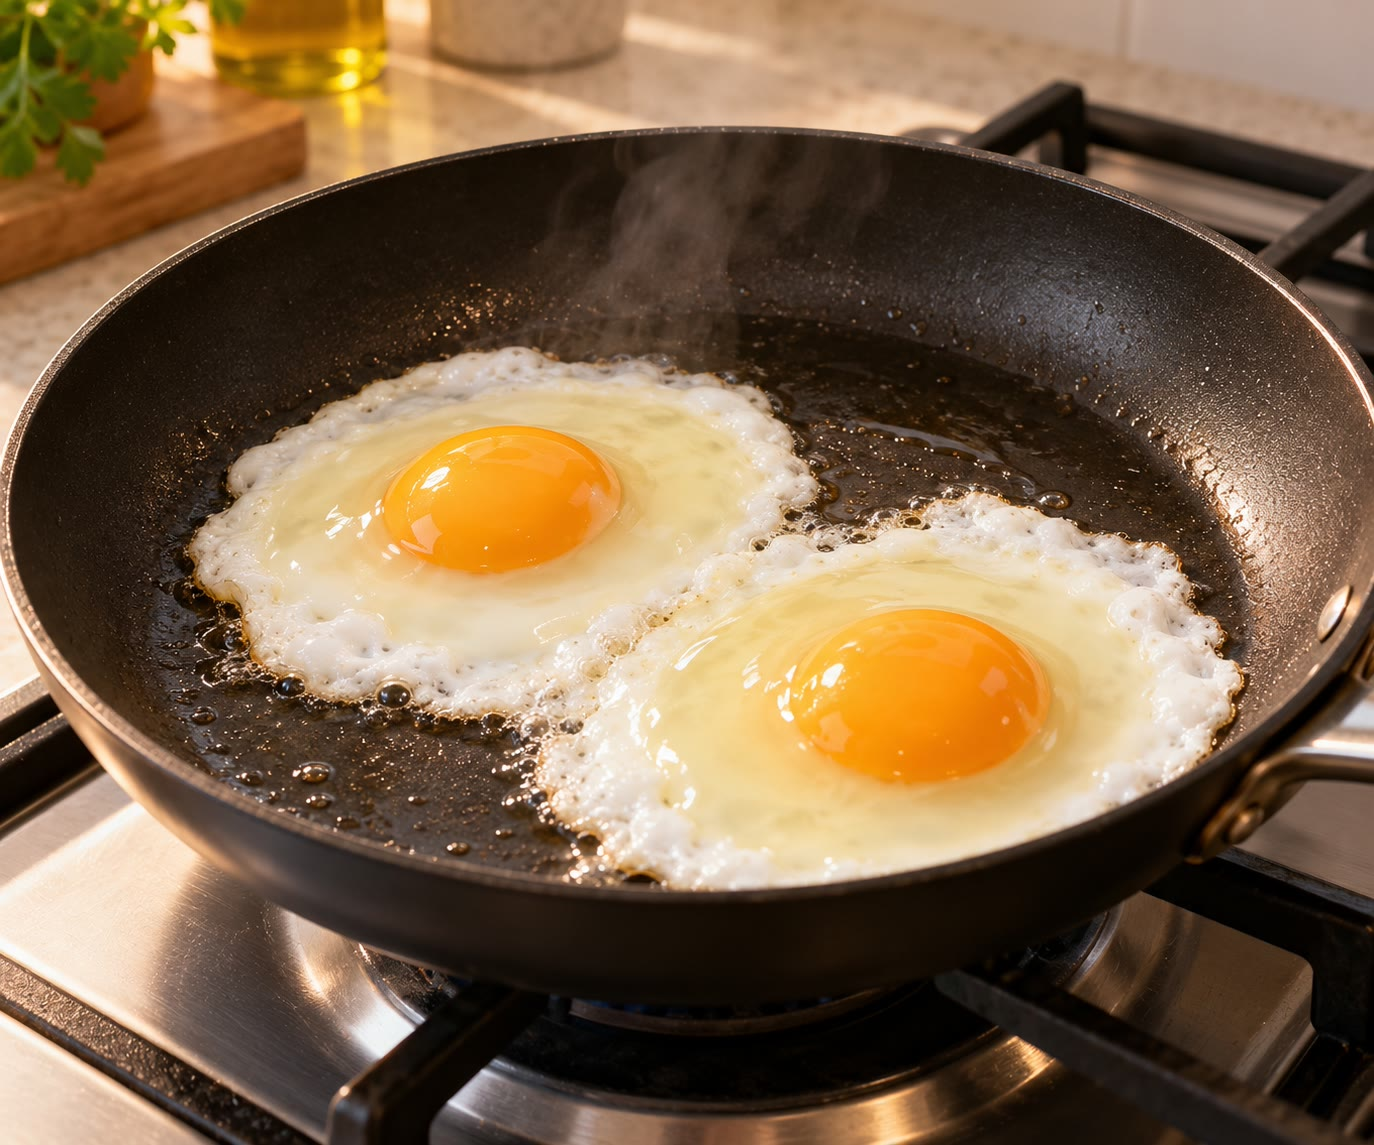
\includegraphics[width=0.5\linewidth]{images/book3/ai/b2-30-eggs.jpg}

{\small 煎蛋。加热时蛋清中的蛋白质展开并相互结合：
半透明的液体变为不透明的白色固体。没有肽键断裂，变化在于链的
折叠方式（示意图）。}
\end{omfigure}

\section{碳水化合物}

\begin{definition}[D 与 L]\label{def:b2:biomolecules:d-l}
糖或氨基酸以费歇尔投影式表示，其氧化程度最高的碳位于顶部。
若距顶部最远的手性碳原子上的 \ce{OH}（对于 $\alpha$-氨基酸，
则为 $\alpha$ 碳上的 \ce{NH2}）指向右侧，则称其为 D 型；指向左侧则为 L 型。
这些标记是将构型与甘油醛比较得到的，它们不是 CIP 标记。
\end{definition}

\begin{definition}[单糖]\label{def:b2:biomolecules:sugar}
\emph{单糖}\index{单糖}是一类多羟基醛或多羟基酮，通常可写作
\ce{C_nH_{2n}O_n}，其中 $n$ 为 3 至 7，且不能水解为更小的糖。\emph{醛糖}\index{醛糖}
在 C1 上具有醛基，\emph{酮糖}\index{酮糖}则具有酮基，
通常位于 C2 上。葡萄糖是一种醛己糖，果糖是一种酮己糖。
\end{definition}

在水中，醛己糖几乎全部以环式存在：C5 上的 \ce{OH} 与醛基加成，形成一个
六元半缩醛环（吡喃糖）。环化过程在 C1 上产生一个新的手性碳原子。

\begin{definition}[异头物]\label{def:b2:biomolecules:anomer}
在\emph{哈沃斯投影式}\index{哈沃斯投影式}中，环状糖的环被画成平面形式，
与纸面垂直，其氧原子位于右后方，取代基位于环的上方或下方。
环。半缩醛碳（醛糖的 C1）即\emph{异头碳}\index{异头碳}；它可以采取的
两种构型给出两个非对映异构体，即\emph{异头物}\index{异头物}：对于 D 型
糖，$\alpha$ 型的异头 \ce{OH} 位于环的下方（与 \ce{CH2OH} 相反），$\beta$ 型则位于上方。在
水中，两种异头物通过开链结构相互转化，新溶解的异头物的旋光度会逐渐变化，
最终趋于平衡值，这种现象称为\emph{变旋}\index{变旋}。
\end{definition}

\begin{omfigure}
\setchemfig{atom sep=1.7em}
\begin{minipage}[c]{0.24\linewidth}\centering
\chemfig{CHO-[6]C(-[4]H)(-[0]OH)-[6]C(-[4,,,2]HO)(-[0]H)-[6]C(-[4]H)(-[0]OH)-[6]C(-[4]H)(-[0]OH)-[6]CH_2OH}
\end{minipage}%
\begin{minipage}[c]{0.37\linewidth}\centering
\begin{tikzpicture}[x=1cm, y=1cm, font=\small]
\coordinate (C4) at (-1.5,0); \coordinate (C3) at (-0.75,-0.65); \coordinate (C2) at (0.75,-0.65);
\coordinate (C1) at (1.5,0); \coordinate (O) at (0.75,0.45); \coordinate (C5) at (-0.75,0.45);
\draw (C5) -- (O) -- (C1); \draw (C4) -- (C5);
\draw[line width=2.2pt] (C4) -- (C3) -- (C2) -- (C1);
\node[fill=white, inner sep=1pt] at (O) {O};
\draw (C5) -- ++(0,0.6) node[above] {\ce{CH2OH}};
\draw (C1) -- ++(0,-0.6) node[below] {OH}; \draw (C1) -- ++(0,0.5) node[above] {H};
\draw (C2) -- ++(0,-0.6) node[below] {OH}; \draw (C3) -- ++(0,0.35) node[above, inner sep=1pt] {OH};
\draw (C4) -- ++(0,-0.6) node[below] {OH};
\node at (0,-2.0) {$\alpha$-D-吡喃葡萄糖};
\end{tikzpicture}
\end{minipage}%
\begin{minipage}[c]{0.37\linewidth}\centering
\begin{tikzpicture}[x=1cm, y=1cm, font=\small]
\coordinate (C4) at (-1.5,0); \coordinate (C3) at (-0.75,-0.65); \coordinate (C2) at (0.75,-0.65);
\coordinate (C1) at (1.5,0); \coordinate (O) at (0.75,0.45); \coordinate (C5) at (-0.75,0.45);
\draw (C5) -- (O) -- (C1); \draw (C4) -- (C5);
\draw[line width=2.2pt] (C4) -- (C3) -- (C2) -- (C1);
\node[fill=white, inner sep=1pt] at (O) {O};
\draw (C5) -- ++(0,0.6) node[above] {\ce{CH2OH}};
\draw (C1) -- ++(0,0.5) node[above] {OH}; \draw (C1) -- ++(0,-0.6) node[below] {H};
\draw (C2) -- ++(0,-0.6) node[below] {OH}; \draw (C3) -- ++(0,0.35) node[above, inner sep=1pt] {OH};
\draw (C4) -- ++(0,-0.6) node[below] {OH};
\node at (0,-2.0) {$\beta$-D-吡喃葡萄糖};
\end{tikzpicture}
\end{minipage}
\par\vspace{6pt}

{\small D-葡萄糖。左：费歇尔投影式表示的开链结构，C5 上的 \ce{OH} 位于右侧（D 型）。中
、右：两种吡喃糖异头物的哈沃斯投影式；费歇尔投影式中右侧的基团
朝下，左侧的基团朝上，C5 上的 \ce{CH2OH} 朝上。两种异头物
仅在 C1 处不同。C2 至 C5 上的氢原子省略。}
\end{omfigure}

\begin{method}[从费歇尔投影式到哈沃斯投影式（D-醛吡喃糖）]\label{met:b2:biomolecules:haworth}
\begin{enumerate}
  \item 画出环，O 位于右后方，C1 位于右侧，然后
        沿前方和左侧顺时针依次为 C2、C3、C4，C5 位于左后方。
  \item 费歇尔投影式中位于右侧的基团朝下，位于左侧的基团朝上。
  \item C5 上（D 系）的 \ce{CH2OH} 朝上。
  \item C1 上的 \ce{OH}：$\alpha$ 型朝下，$\beta$ 型朝上。
\end{enumerate}
\end{method}

\begin{proposition}[变旋平衡]\label{prop:b2:biomolecules:mutarotation}
设纯异头物的比旋光度分别为 $[\alpha]_\alpha$ 与 $[\alpha]_\beta$，平衡混合物的
比旋光度为 $[\alpha]_{\mathrm{eq}}$，则平衡时 $\alpha$ 异头物的
摩尔分数为
\begin{equation*}
x_\alpha = \frac{[\alpha]_{\mathrm{eq}} - [\alpha]_\beta}{[\alpha]_\alpha - [\alpha]_\beta}.
\end{equation*}
\end{proposition}

\begin{proof}
开链在混合物中所占比例极小，可以忽略。两种异头物的旋光度
按其浓度成比例相加（毕奥定律，见本科一年级分册）；由于二者摩尔质量相同，
有 $[\alpha]_{\mathrm{eq}} = x_\alpha[\alpha]_\alpha + (1 - x_\alpha)[\alpha]_\beta$，
由此解出 $x_\alpha$。
\end{proof}

平衡状态下水中的 D-葡萄糖，$[\alpha] = +52.7$（单位为 \unit{\degree\,dm^{-1}\,g^{-1}\,mL}）。
已知两种异头物的旋光度分别为 $+112$ 与 $+18.7$（练习数据），则 $x_\alpha = (52.7 - 18.7)/(112 - 18.7)
\approx 0.36$：约 36~\% 为 $\alpha$ 型，64~\% 为 $\beta$ 型。$\beta$ 异头物的所有取代基
在椅式构象中均为平伏键，因而更稳定。
% ledger: rot:glucose-eq

\begin{definition}[糖苷]\label{def:b2:biomolecules:glycoside}
\emph{糖苷}\index{糖苷}是糖的异头 \ce{OH}
被醇中的 \ce{OR} 基团取代后形成的缩醛，醇常为另一个糖分子；异头碳到该
氧原子之间的键称为\emph{糖苷键}\index{糖苷键}。\emph{还原糖}\index{还原糖}是
能够还原弱氧化剂（如斐林试剂或托伦试剂）的糖。
\end{definition}

\begin{proposition}[是否具有还原性]\label{prop:b2:biomolecules:reducing}
含有游离半缩醛（或半缩酮）基团的糖具有还原性；若糖苷的异头碳
均参与糖苷键的形成，则不具有还原性。
\end{proposition}

\begin{proof}[论证]
半缩醛与开链结构处于平衡之中，其醛基会被试剂氧化；
平衡随之使更多的环打开，直至糖全部反应。缩醛在
中性或碱性水溶液中不开环：异头碳保持封闭，没有可被氧化的醛基。
\end{proof}

麦芽糖由两个葡萄糖构成（其中一个的 C1 与另一个的 O4 相连），保留一个游离半缩醛基团，因而具有还原性；
蔗糖则是葡萄糖与果糖的异头碳彼此相连，不具有还原性。淀粉与
纤维素均为葡萄糖通过 C1--O4 连接而成的链：淀粉中为 $\alpha$ 型，链卷曲且可被消化；
纤维素中为 $\beta$ 型，其直链通过氢键堆积成纤维。

\section{脂质}

\begin{definition}[脂质]\label{def:b2:biomolecules:lipid}
\emph{脂肪酸}\index{脂肪酸}是具有长而无支链碳链的羧酸，通常含 12 至
22 个碳原子，可为饱和的，也可含（\textit{Z}）双键。\emph{三酰甘油}\index{三酰甘油}是
丙-1,2,3-三醇（甘油）与三个脂肪酸形成的三酯。
\emph{磷脂}\index{磷脂}是甘油与两个脂肪酸形成的二酯，其第三位
连有磷酸基团，该磷酸基团再与一个小的极性基团相连。
\end{definition}

（\textit{Z}）双键使碳链弯折，从而难以紧密堆积：硬脂酸（18 个碳，
饱和）在 \qty{69}{\degreeCelsius} 时熔化，油酸（18 个碳，含一个 \textit{Z} 双键）在
\qty{13}{\degreeCelsius} 时熔化。富含饱和链的脂肪在室温下为固体；富含不饱和链的油
则为液体。三酰甘油经皂化生成甘油与肥皂
（见\cref{ch:b2:acyl-substitution}）。
% ledger: mp:stearic, mp:oleic

\begin{omfigure}
\begin{tikzpicture}[x=1cm, y=1cm]
\foreach \i in {0,1,2,3,4,5,6,7,8,9}{
  \fill[omDef!60] (0.6*\i,1.6) circle (0.17);
  \draw[thick, black!70] (0.6*\i-0.06,1.43) .. controls (0.6*\i-0.12,1.2) and (0.6*\i,1.0) .. (0.6*\i-0.06,0.75);
  \draw[thick, black!70] (0.6*\i+0.06,1.43) .. controls (0.6*\i+0.12,1.2) and (0.6*\i,1.0) .. (0.6*\i+0.06,0.75);
  \fill[omDef!60] (0.6*\i,-0.6) circle (0.17);
  \draw[thick, black!70] (0.6*\i-0.06,-0.43) .. controls (0.6*\i-0.12,-0.2) and (0.6*\i,0.0) .. (0.6*\i-0.06,0.25);
  \draw[thick, black!70] (0.6*\i+0.06,-0.43) .. controls (0.6*\i+0.12,-0.2) and (0.6*\i,0.0) .. (0.6*\i+0.06,0.25);
}
\node[font=\small, anchor=west] at (6.0,2.2) {水};
\node[font=\small, anchor=west] at (6.0,0.5) {烃类内核};
\node[font=\small, anchor=west] at (6.0,-1.2) {水};
\draw[densely dotted] (5.6,1.6) -- (6.0,1.6) node[right, font=\footnotesize] {极性头部};
\draw[densely dotted] (5.6,1.05) -- (6.0,1.05) node[right, font=\footnotesize] {两条脂肪酸尾链};
\end{tikzpicture}
\par\vspace{4pt}

{\small 磷脂双分子层示意图：两侧的极性头部面向水，
烃尾在内部相接。细胞膜即建立在此结构之上；每个头部仅连一条烃尾的肥皂则形成小球，尾部朝内，称为
胶束。}
\end{omfigure}

\section{核苷酸}

\begin{definition}[核苷酸]\label{def:b2:biomolecules:nucleotide}
\emph{碱基}\index{碱基}是含氮杂环化合物：腺嘌呤（A）与鸟嘌呤（G）为嘌呤；
胞嘧啶（C）、胸腺嘧啶（T）与尿嘧啶（U）为嘧啶。\emph{核苷}\index{核苷}是
碱基通过一个氮原子与核糖或 2-脱氧核糖的 C1 相连所形成的化合物（即 $N$-糖苷）。
\emph{核苷酸}\index{核苷酸}是核苷的磷酸酯。在核酸中，
核苷酸之间通过\emph{磷酸二酯键}\index{磷酸二酯键}相连：一个磷酸基团连接
一个糖的 O3 与下一个糖的 O5。
\end{definition}

DNA 使用 2-脱氧核糖以及碱基 A、G、C、T；RNA 使用核糖，并以 U 代替 T。核酸链具有
一定的方向，由其 5$'$ 端指向 3$'$ 端；磷酸基团在生理 pH 下电离，使链成为
聚阴离子。两条 DNA 链方向相反，依靠彼此相对的碱基之间的
氢键结合在一起。

\begin{proposition}[碱基配对]\label{prop:b2:biomolecules:pairing}
在双链 DNA 中，腺嘌呤通过两个氢键与胸腺嘧啶配对，鸟嘌呤
与胞嘧啶通过三个氢键配对。
\end{proposition}

\begin{proof}[论证]
配对的条件是：边缘的供体（\ce{N-H}）与受体（\ce{C=O} 的氧、环上的
氮）位于合适的距离，并使嘌呤与嘧啶相对，从而每一对宽度相同。
A 提供 \ce{N-H}（其氨基）和一个环上的 \ce{N}；T 提供 \ce{C=O} 和 \ce{N-H}：两个氢键。G
提供 \ce{C=O}、\ce{N-H} 和 \ce{N-H}（氨基）；C 提供 \ce{N-H}（氨基）、\ce{N} 和 \ce{C=O}：三个
氢键。图中给出了这些配对。
\end{proof}

\begin{omfigure}
\setchemfig{atom sep=1.7em}
\chemfig{?[a](-[:90]CH_3)-[:-30](=[:30]@{to}O)-[:-90]N(-[:-30]@{th}H)-[:-150](=[:-90]O)-[:150]N(-[:-150]R)-[:90]?[a,2]}%
\hspace{2.3em}%
\raisebox{-1.0em}{\chemfig{?[a](-[:150]N(-[:90]H)-[:210]@{ah}H)-[:30]?[b](-[:78]N=[:6]-[:-66]N(-[:-30]R)-[:-138]?[c])=[:-30]?[c]-[:-90]N=[:-150]-[:150]@{an}N?[a,2]}}
\chemmove{\draw[-, densely dotted, thick](to)--(ah); \draw[-, densely dotted, thick](th)--(an);}
\hspace{1.5em}
\chemfig{?[a]-[:-30](-[:30]N(-[:90]H)-[:-30]@{ch}H)=[:-90]@{cn}N-[:-150](=[:-90]@{co}O)-[:150]N(-[:-150]R)-[:90]?[a,2]}%
\hspace{2.3em}%
\raisebox{-0.6em}{\chemfig{?[a](=[:150]@{go}O)-[:30]?[b](-[:78]N=[:6]-[:-66]N(-[:-30]R)-[:-138]?[c])=[:-30]?[c]-[:-90]N=[:-150](-[:-90]N(-[:-30]H)-[:-150]@{gh}H)-[:150]N?[a](-[:180]@{gn}H)}}
\chemmove{\draw[-, densely dotted, thick](ch)--(go); \draw[-, densely dotted, thick](cn)--(gn);
  \draw[-, densely dotted, thick](co)--(gh);}
\par\vspace{6pt}

{\small DNA 的两种碱基对。左：胸腺嘧啶与腺嘌呤，两个氢键（虚线）。右：
胞嘧啶与鸟嘌呤，三个氢键。R 为每条链的脱氧核糖；一对碱基中的两个 R 基团指向
同一侧，朝向两条主链。}
\end{omfigure}

\begin{history}[糖的构型，1891 年]
\begin{minipage}[t]{0.18\linewidth}
\vspace{0pt}
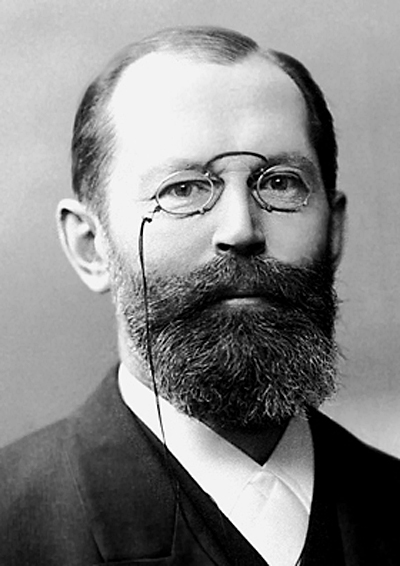
\includegraphics[width=\linewidth]{images/book3/fischer.jpg}
\end{minipage}\hfill
\begin{minipage}[t]{0.78\linewidth}
\vspace{0pt}
埃米尔·费歇尔于 1891 年前便确定了葡萄糖及其同分异构体的构型，
他通过糖之间相互转化，并统计所得
立体异构体的数目。他为书写这些结构所发明的投影式至今仍以他的名字命名。他还合成了首批
肽，并于 1902 年获得诺贝尔化学奖。（肖像：Atelier
Victoria, Berlin，约 1895 年，公有领域；维基共享资源。）
\end{minipage}
\end{history}

\section{练习}

\begin{exercise}[$\star$]\label{exo:b2:biomolecules:1}
画出丙氨酸的两性离子形式，再画出在 pH 1 和 pH 12 时占主导的形式。
\end{exercise}

\begin{exercise}[$\star$]\label{exo:b2:biomolecules:2}
求甘氨酸的等电点，以及丙氨酸的等电点（$\mathrm pK_a$ 为 2.35 和 9.87）。
\end{exercise}

\begin{exercise}[$\star$]\label{exo:b2:biomolecules:3}
画出二肽 Ala--Gly，并圈出其肽键。它与 Gly--Ala 有何不同？
\end{exercise}

\begin{exercise}[$\star$]\label{exo:b2:biomolecules:4}
在费歇尔投影式中，顶端为 \ce{COOH}，底端为侧链 \ce{CH2OH}，
丝氨酸的 \ce{NH2} 指向左侧。它属于 D 型还是 L 型？给出其 CIP 标记。
\end{exercise}

\begin{exercise}[$\star\star$]\label{exo:b2:biomolecules:5}
求三肽 Lys--Gly--Asp 在 pH 1、7 和 12 时的净电荷。
\end{exercise}

\begin{exercise}[$\star\star$]\label{exo:b2:biomolecules:6}
为什么形成肽键要用偶联剂，而不用受保护的氨基
酸经亚硫酰氯处理并加热所得的酰氯？
\end{exercise}

\begin{exercise}[$\star\star$]\label{exo:b2:biomolecules:7}
D-果糖通过其 C5 上的 \ce{OH} 与 C2 酮基环化。给出所成环的大小，并以
哈沃斯投影式画出 $\beta$-D-呋喃果糖。
\end{exercise}

\begin{exercise}[$\star\star$]\label{exo:b2:biomolecules:8}
D-半乳糖两种纯异头物的比旋光度分别为 $+150.7$（$\alpha$）和 $+52.8$（$\beta$），
平衡混合物的比旋光度为 $+80.2$（题给数据）。求平衡时的组成。
\end{exercise}

\begin{exercise}[$\star\star$]\label{exo:b2:biomolecules:9}
解释为什么麦芽糖能还原斐林试剂而蔗糖不能，
以及为什么蔗糖经稀酸加热后却能还原斐林试剂。
\end{exercise}

\begin{exercise}[$\star\star\star$]\label{exo:b2:biomolecules:10}
油脂的皂化值是皂化 1~g 油脂所需氢氧化钾的质量，以 mg 计。
求三油酸甘油酯（\ce{C57H104O6}）的皂化值，并解释为何链较短的油脂皂化值更高。
\end{exercise}

\begin{exercise}[$\star\star\star$]\label{exo:b2:biomolecules:11}
以甘氨酸和丙氨酸为原料，规划 Gly--Ala 的合成：使用保护基、活化、偶联，
脱保护，并选用一对正交保护基。
\end{exercise}

\begin{exercise}[$\star\star\star$]\label{exo:b2:biomolecules:12}
写出与 5$'$-ATGCGT-3$'$ 互补的链（自其 5$'$ 端写起），并统计
维系该双链的氢键数目。
\end{exercise}

\section{问题：阿斯巴甜}

\begin{problem}[{周末问题——两种氨基酸及其构型，二肽的电荷随 pH
的变化，其合成与 $\alpha$/$\beta$ 问题，以及其在软
饮料中的水解}]
\label{pb:b2:biomolecules:1}
阿斯巴甜是 L-天冬氨酸的 $\alpha$-羧基
与 L-苯丙氨酸的氨基缩合形成的二肽的甲酯。数据：天冬氨酸的 $\mathrm pK_a$ 为 2.0、3.9 和 9.9（模型
值，对应二肽中的各基团）。摩尔质量（\unit{g/mol}）：C 12.011、H 1.008、N 14.007、
O 15.999。
% ledger: use:aspartame, pka:asp1, pka:asp2, pka:asp3, aw:C, aw:H, aw:N, aw:O

\medskip
\noindent\textbf{第一部分——两种氨基酸。}
\begin{enumerate}
  \item 写出阿斯巴甜完全水解所释放的三种化合物的名称。
  \item 用费歇尔投影式画出 L-天冬氨酸和 L-苯丙氨酸。
  \item 给出每个手性碳原子的 CIP 描述符。
  \item 阿斯巴甜有多少种立体异构体？
  \item 画出阿斯巴甜的结构，并标出肽键和酯基。
  \item 为什么每种氨基酸的构型对甜味至关重要？
\end{enumerate}

\medskip
\noindent\textbf{第二部分——电荷随 pH 的变化。}
\begin{enumerate}[resume]
  \item 列出阿斯巴甜中可电离的基团。为什么 C 端不是其中之一？
  \item 取模型值，求 pH 为 2 时的净电荷。
  \item 同上，求 pH 为 7 时的净电荷。
  \item 同上，求 pH 为 12 时的净电荷。
  \item 在此模型下估算等电点。
  \item 为什么二肽的真实 $\mathrm pK_a$ 值会不同于
        游离天冬氨酸的数值？
\end{enumerate}

\medskip
\noindent\textbf{第三部分——合成。}
\begin{enumerate}[resume]
  \item 为什么不能简单地将天冬氨酸与苯丙氨酸甲酯直接加热？
  \item 天冬氨酸的哪些基团必须加以保护？
  \item 偶联剂对游离的羧基有何作用？
  \item 天冬氨酸含有两个羧基。若偶联了错误的那个羧基，会生成什么？
  \item 提出一种正交保护方案，使仅 $\alpha$-羧基保持游离，并给出
        其脱保护的方法。
  \item 为什么活化后的氨基酸不能在碱性条件下放置过久？
  \item 写出各步骤的顺序。
\end{enumerate}

\medskip
\noindent\textbf{第四部分——软饮料中的水解。}
\begin{enumerate}[resume]
  \item 阿斯巴甜的哪些键可在酸性饮料中水解？哪一个先断裂？
  \item 仅考虑酯基的水解，给出其水解产物。
  \item 为什么放置久的饮料甜味变淡？
  \item 计算阿斯巴甜 \ce{C14H18N2O5} 的摩尔质量。
  \item 计算一罐中含 \qty{180}{mg} 阿斯巴甜的物质的量。
  \item 给出 \qty{180}{mg} 阿斯巴甜完全水解
        时释放的甲醇质量。
\end{enumerate}
\end{problem}
